\section*{Design}

\subsection*{Mockup}

\begin{figure}
    \centering
    
\includegraphics[width=0.8\textwidth]{res/login.png}
    \caption{Schermata di login}
    \label{fig:mockup}
\end{figure}

\begin{figure}
    \centering
    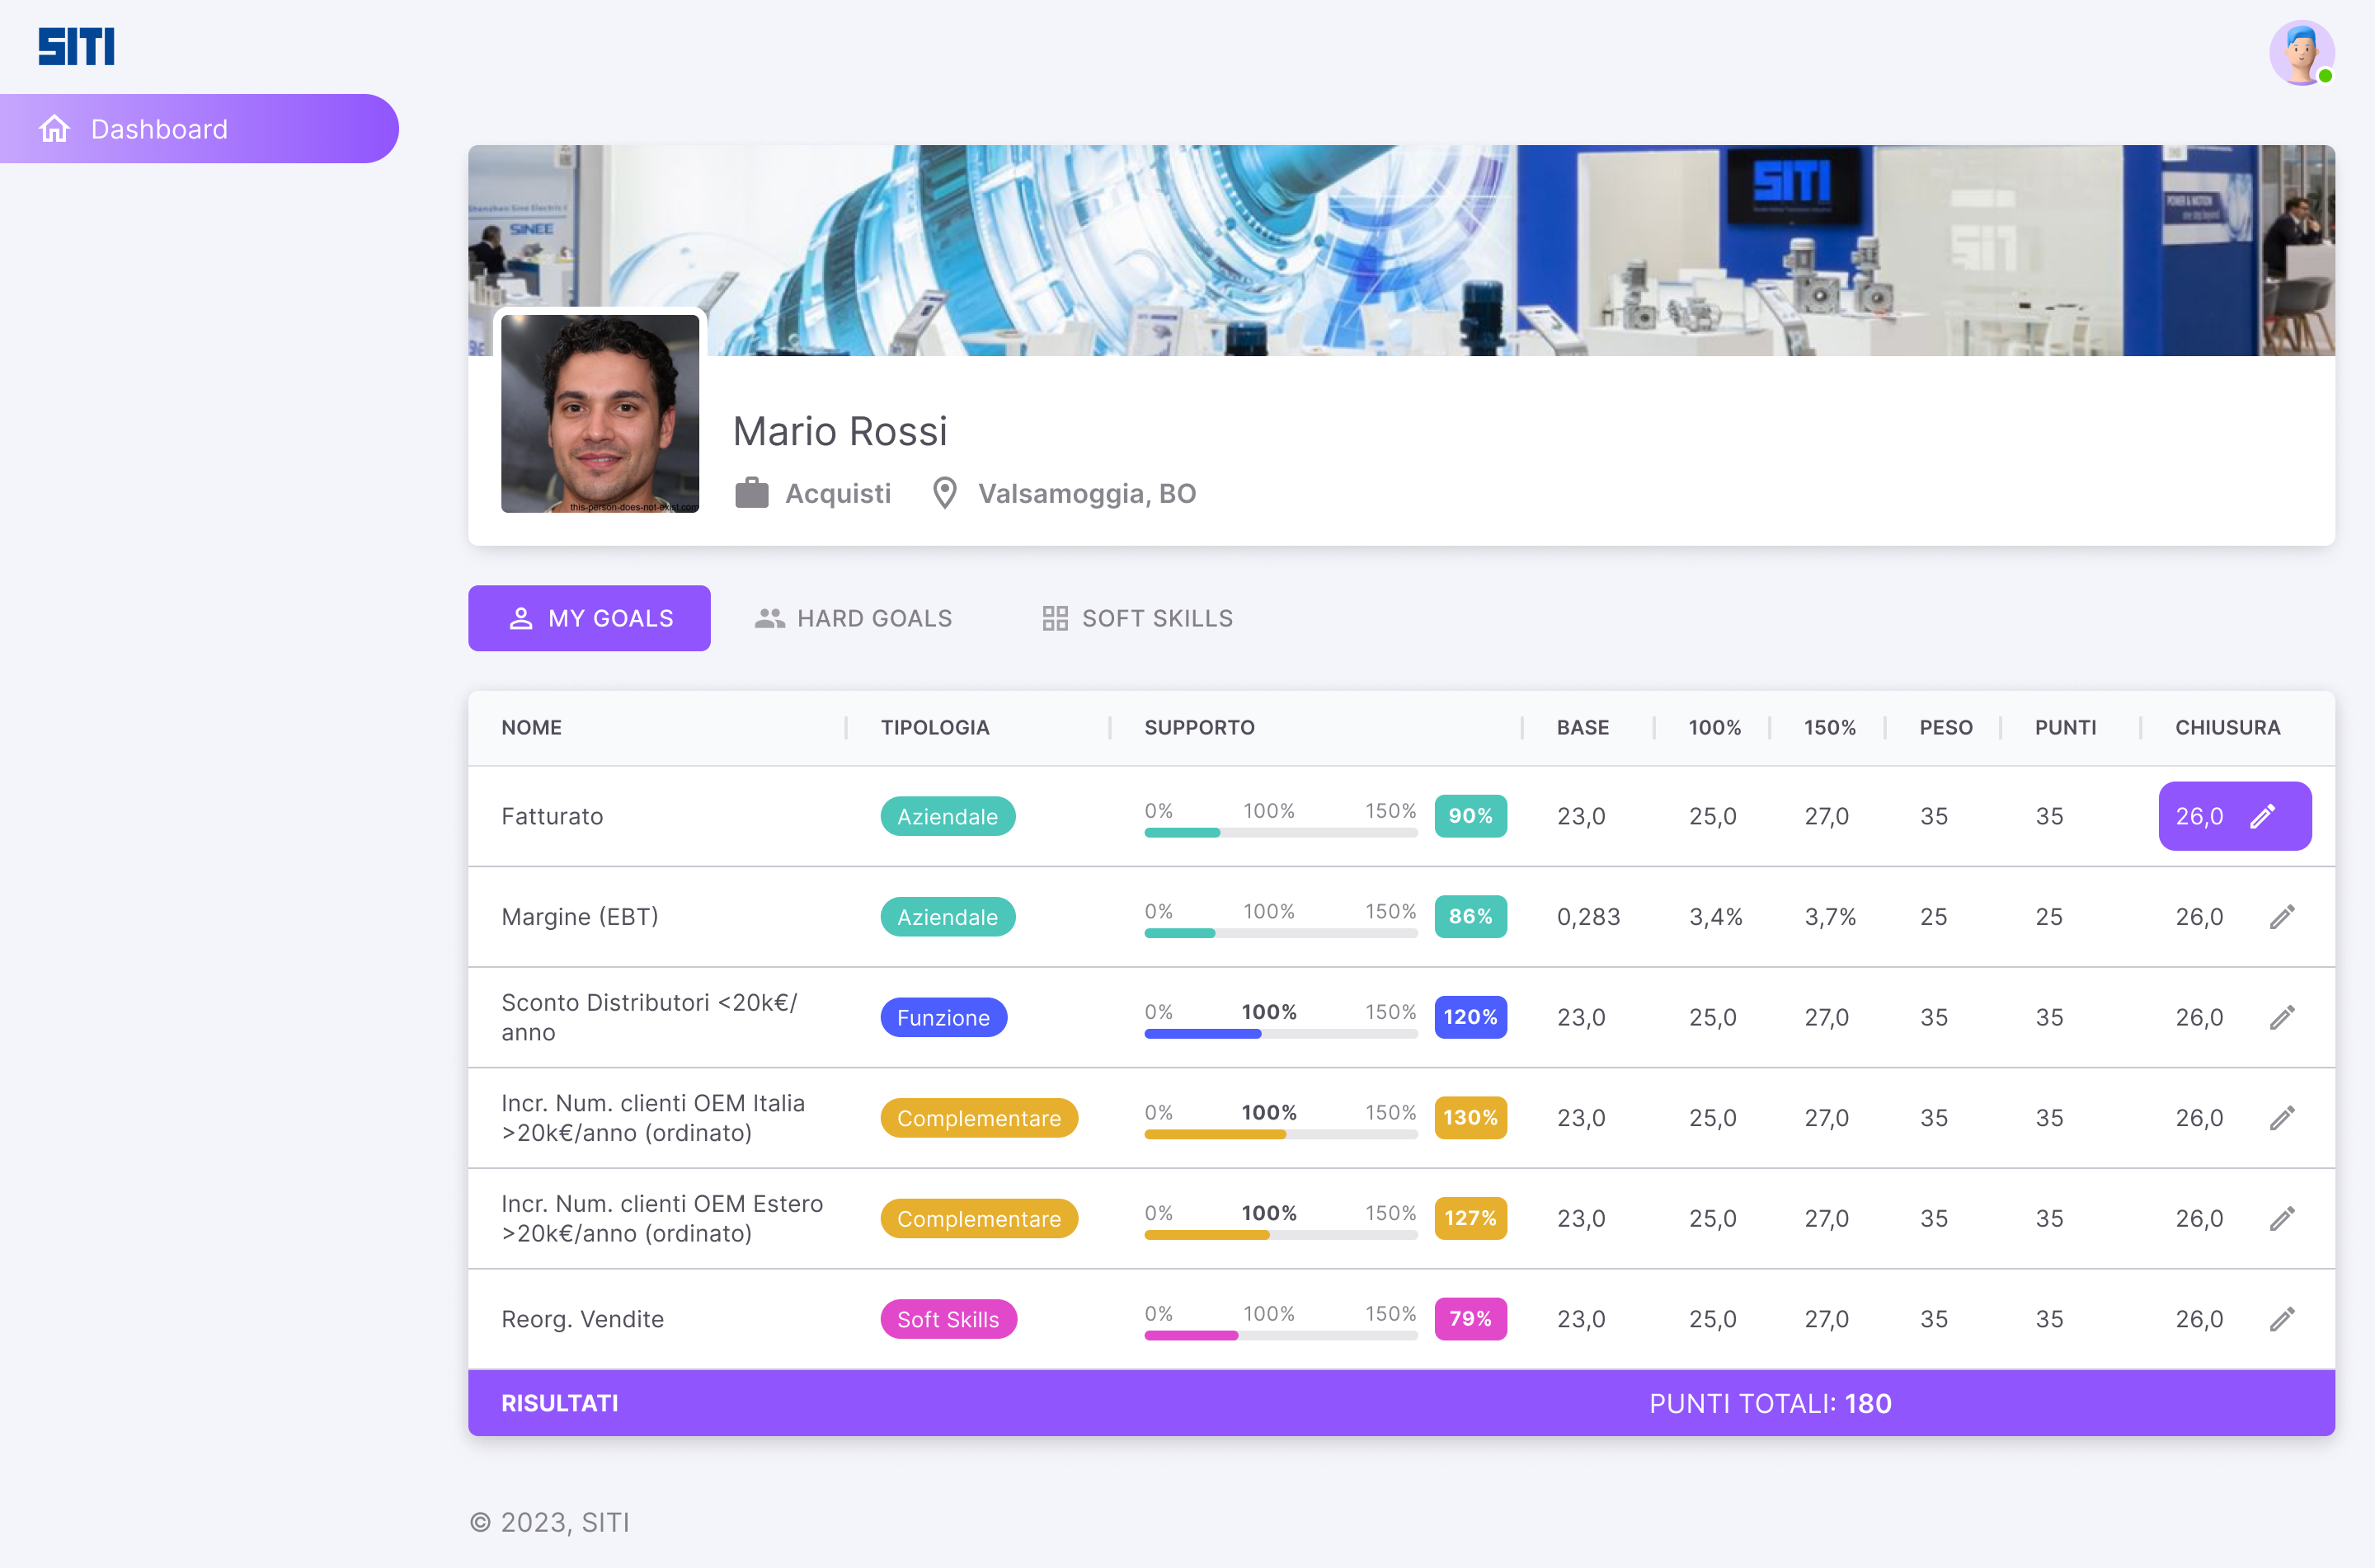
\includegraphics[width=0.8\textwidth]{res/dashboard.png}
    \caption{Dipendente - dashboard dei propri obiettivi}
    \label{fig:mockup}
\end{figure}

\begin{figure}
    \centering
    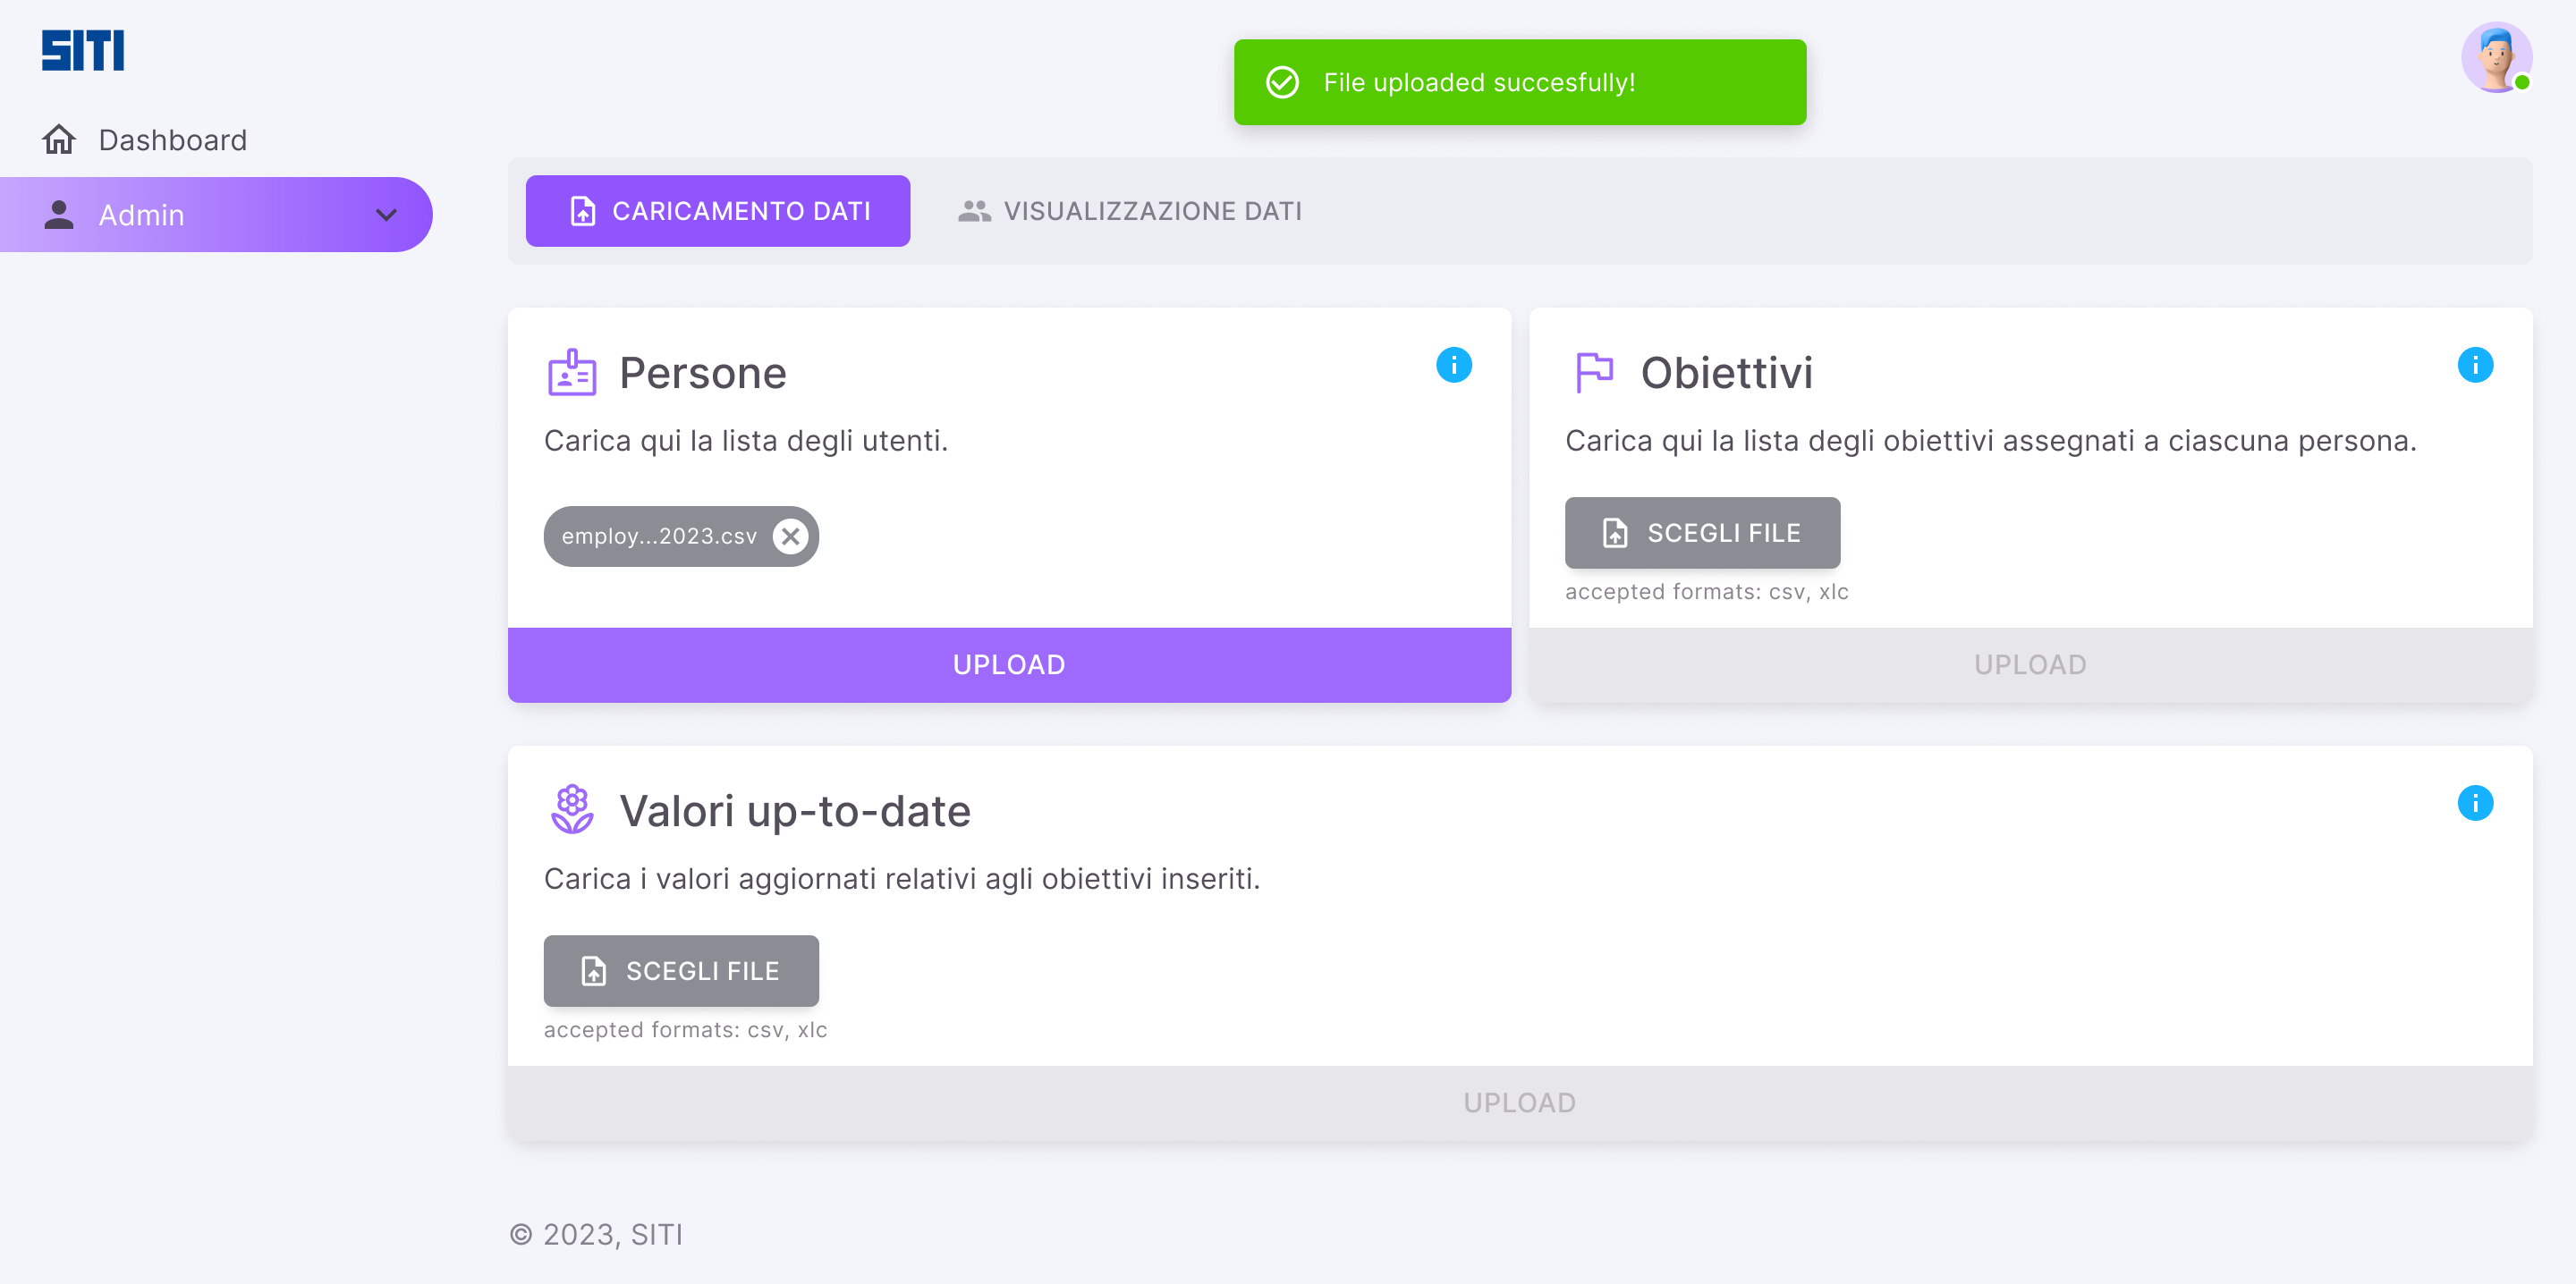
\includegraphics[width=0.8\textwidth]{res/upload.png}
    \caption{Admin - upload dei dati in formato csv}
    \label{fig:mockup}
\end{figure}

\begin{figure}
    \centering
    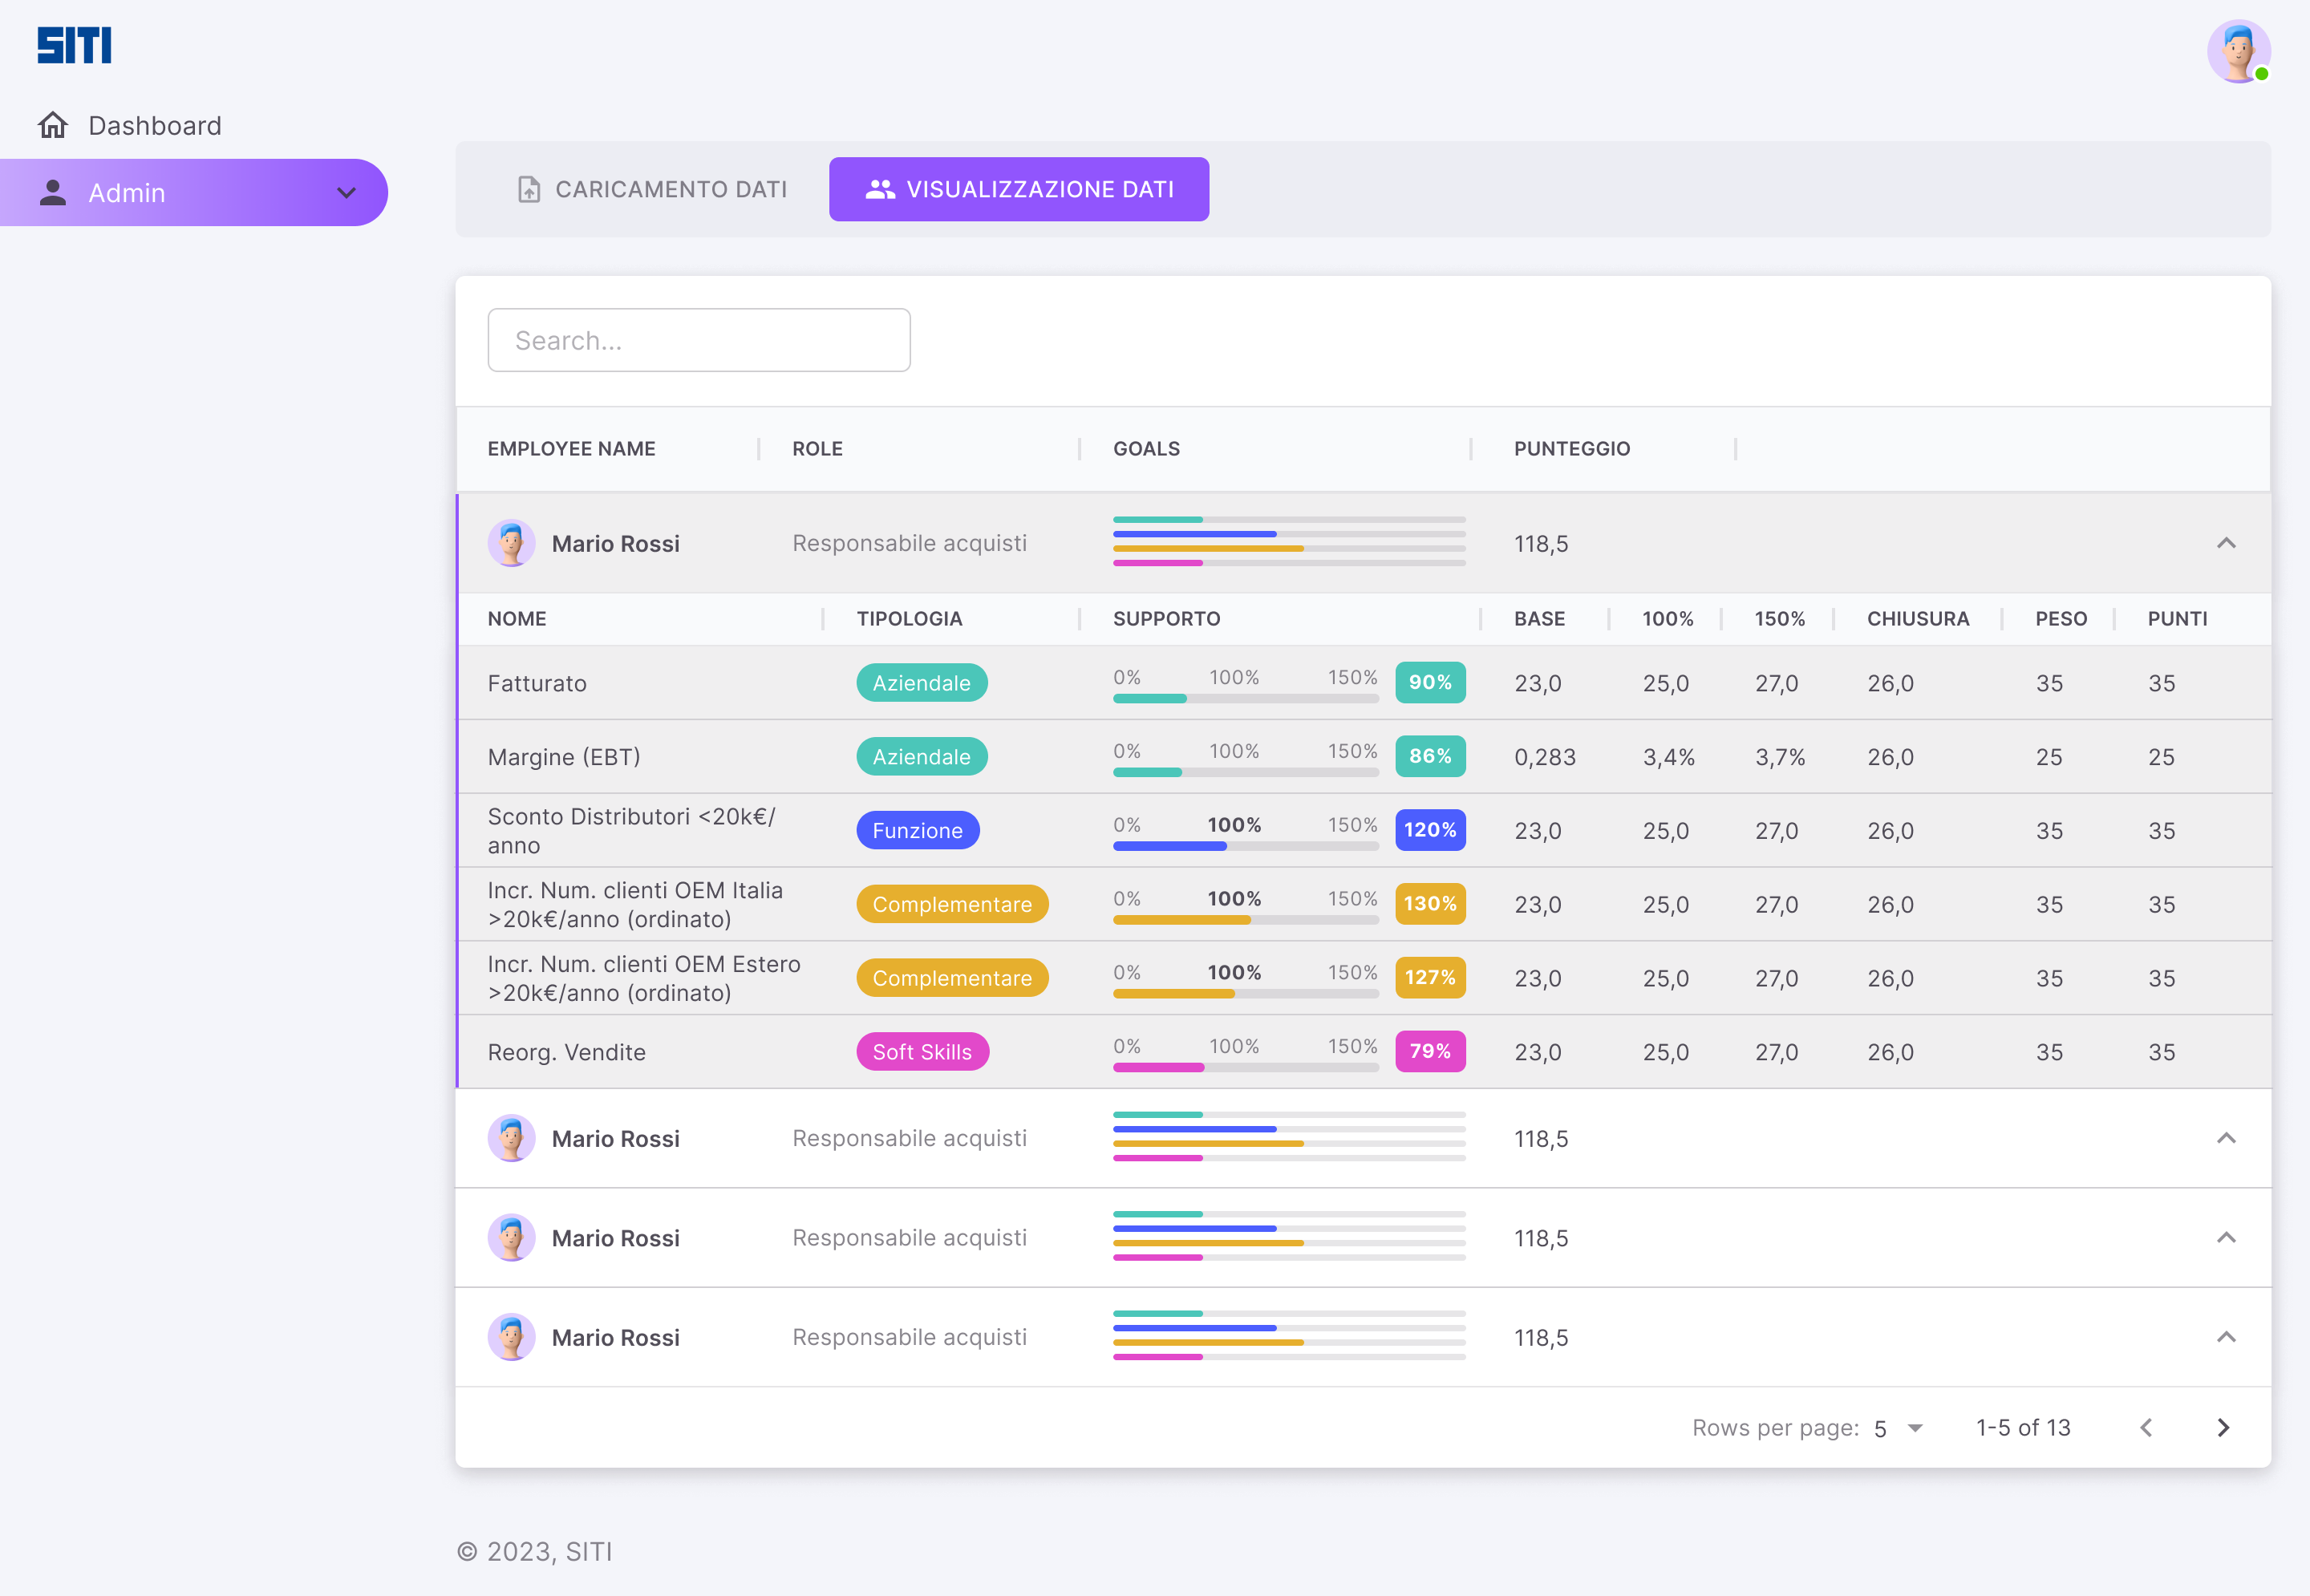
\includegraphics[width=0.8\textwidth]{res/dati.png}
    \caption{Admin - visione d'insieme su tutti i dipendenti}
    \label{fig:mockup}
\end{figure}


Il valore di chiusura è il valore raggiunto per l'obiettivo a fine anno. Di default è pari al valore base per l'anno corrente, finchè i dati up-to-date non vengono inseriti.
Nei mockup non era stata prevista la colonna up-to-date. Il design finale dell'app consiste in:
\begin{itemize}
    \item l'admin vede i valori up-to-date di ciascun dipendente
    \item i dipendenti nella propria dashboard, oltre alla colonna up-to-date, hanno a disposizione anche la colonna "chiusura", che è modificabile e consente di simulare valori possibili di chiusura e vedere come cambierebbe il punteggio.
\end{itemize}



\subsection*{Architettura}